\documentclass[11pt]{article}
\usepackage[utf8]{inputenc}
\usepackage[T1]{fontenc}
\usepackage{amsmath,amssymb,amsthm}
\usepackage{booktabs}
\usepackage[margin=2.6cm]{geometry}
\usepackage{xcolor}
\usepackage{pgfplots}
\usepgfplotslibrary{groupplots}
\pgfplotsset{compat=1.16}
\definecolor{serieA}{HTML}{2A78D6}
\definecolor{serieB}{HTML}{EB6834}
\usepackage[colorlinks=true,linkcolor=blue!50!black,citecolor=blue!50!black,urlcolor=blue!50!black]{hyperref}

% Notas de trabajo: se apagan cambiando \todo por un comando vacio.
\newcommand{\todo}[1]{{\color{red!70!black}\textbf{[TODO:} #1\textbf{]}}}

% Notacion
\newcommand{\iv}[1]{\mathbf{#1}}          % intervalo o caja
\newcommand{\R}{\mathbb{R}}
\newcommand{\IR}{\mathbb{IR}}
\newcommand{\Abar}{\bar{A}}
\newcommand{\inff}{\operatorname{inf}}
\newcommand{\supp}{\operatorname{sup}}
\newcommand{\wid}{\operatorname{wid}}
\newcommand{\magn}{\operatorname{mag}}

\newtheorem{proposition}{Proposition}
\newtheorem{lemma}[proposition]{Lemma}
\newtheorem{corollary}[proposition]{Corollary}
\theoremstyle{definition}
\newtheorem{definition}[proposition]{Definition}
\theoremstyle{remark}
\newtheorem{remark}[proposition]{Remark}

\title{A self-certifying simplex for rigorous\\ polytope-hull contraction in interval branch and bound}
\author{Ignacio Araya \and \todo{coautores}}
\date{\todo{borrador del 2026-10-10}}

\begin{document}
\maketitle

% =====================================================================
\begin{abstract}
Polytope-hull contractors bound each variable of an interval branch-and-bound
node over a linear relaxation by solving $2n$ linear programs. Current
implementations delegate them to a floating-point LP solver and recover rigor
afterwards from its dual solution. These LPs are small and two or three pivots
apart, so a general-purpose solver spends more per call on setting up,
refactorizing and verifying than on pivoting. We present a self-certifying
simplex (SC) designed around the certificate instead: writing the relaxation
as $\Abar z=0$ with interval-bounded slacks, any basis yields a valid bound on
the box and every sub-box, so SC needs no verification, no refactorization
before declaring an optimum and no phase~1; the $2n$ problems share one
tableau, with a warm start chosen per program and a hybrid tableau/revised
engine. Replaying the same polytope-hull passes inside the same contractor,
with the same contraction, a pass of SC costs 0.56--0.62 times that of SoPlex
as used by Ibex, 0.72--0.80 times that of its bare simplex driven directly,
and 0.12--0.26 times that of HiGHS and Gurobi. An emulation attributes the
remaining gap to the refactorization and verification that the certificate
makes unnecessary. Where the LP solver ends without an optimum, SC still
certifies the bound. The whole solver is 13--15\% faster on 240 global
optimization problems and 7--8\% faster on 242 systems of equations, with
slightly fewer cells, and SC never exceeds the LP hull beyond the tolerance of
an LP oracle.
\end{abstract}

% =====================================================================
\section{Introduction}\label{sec:intro}

Interval branch-and-bound solvers compute, with mathematical certainty, an
enclosure of all solutions of a system of nonlinear equations and inequalities,
or the global optimum of a constrained problem~\cite{neumaier2004complete}.
Their efficiency depends on \emph{contractors}, operators that shrink the
current box without losing solutions~\cite{chabert2009contractor}. Among them,
contractors based on linear relaxations are among the most effective: the
constraints are linearized over the box, by convex interval
Taylor forms~\cite{araya2012xnewton} or affine
arithmetic~\cite{ninin2015affine,araya2025hybridizing}, and each variable is
minimized and maximized over the resulting polytope. In Ibex this is the
polytope-hull contractor, the linear part of X-Newton, which we introduced
in~\cite{araya2012xnewton}; we later combined the affine and Taylor-based
relaxations~\cite{araya2025hybridizing}.

Each call solves up to $2n$ linear programs, and the rigor of the result cannot
come from the LP solver, which works in floating point. Current implementations
therefore treat the LP solver as a black box and certify its output a
posteriori: the dual solution is turned into a safe bound by the
Neumaier--Shcherbina procedure~\cite{neumaier2004safe}, and an infeasibility
claim is accepted only if the returned Farkas ray passes the same verification.
This design has two costs. The first is easy to miss and turns out to be the
larger one: the $2n$ LPs of a node are small and closely related, typically
two or three pivots apart, and each is a separate call to a general-purpose
solver, which sets up its vectors, refactorizes the basis before declaring an
optimum and verifies its solution; on these LPs that work exceeds the pivots
themselves (Section~\ref{sec:experiments}). The second is in the bounds. When
the verification fails, which happens when the dual is inaccurate or the
solver works in an unfavourable representation, the bound is lost; when the
solver reports infeasibility without a verifiable ray, the pass is abandoned
and the node survives. On our benchmark these losses, and not the quality of
the relaxation, explain most of the pruning gap between contractors that share
the same polytope (Section~\ref{sec:experiments}).

\paragraph{Positioning.} The certificate we use is not new. That \emph{any}
multiplier vector yields a valid bound once the residual is evaluated in
interval arithmetic is the principle of Neumaier and
Shcherbina~\cite{neumaier2004safe}. Domes and Neumaier~\cite{domes2012rigorous}
applied it to filtering with linear relaxations: they solve the bound LPs with
an external solver, collect the multipliers, and solve the preconditioned
interval system row by row. In previous work~\cite{reyes2023preconditioning} we
wrote the relaxation in the homogeneous form used here, with one auxiliary
variable per row, and showed that the optimal preconditioner for an interval
Gauss--Seidel projection is given by the dual solutions of the bound LPs; the
equivalent valid inequalities appear in the optimization-based bound
tightening of Gleixner et al.~\cite{gleixner2017three}, and both works reuse
them in sub-boxes. The present paper continues that line: there the
multipliers were still computed by an external LP solver, and the
preconditioner was recomputed only periodically to amortize its cost. On the solver side, Yamamura and
coworkers~\cite{yamamura2001dual,yamamura2006dual} observed that, after a
bisection, the optimal tableau of the parent remains dual feasible for the
child, so that an LP emptiness test can be resumed by the dual simplex method
with few or no pivots per box.

What changes with a self-certifying simplex is \emph{where the multipliers come from and how often a
usable certificate is available}. In the approaches above, multipliers are a
by-product of an external solver and certification is a post-processing step;
its cost and fragility lead to applying it to a few promising
variables~\cite{domes2012rigorous}, to recomputing it only periodically and
reusing it in between~\cite{reyes2023preconditioning}, or to abandoning the pass
when it fails (Ibex). The dual-simplex warm start of Yamamura et al.\ concerns a
single feasibility LP on a fixed relaxation, without rigorous certification.
The self-certifying simplex is designed for the certificate: in the homogeneous form every
basis can be made dual feasible by relocating nonbasic variables, so each of the
$2n$ bound problems, and each problem after the box contracts, starts dual
feasible; the $2n$ problems share one tableau; and the multipliers of the
current basis give a valid certificate at every bound and, with the dual
method, at every iteration. Bound tightening by optimization is also central in
MINLP solvers~\cite{belotti2009branching,gleixner2017three}, where rigor is not
required; the heuristic of skipping bounds already attained by a primal point,
used by Ibex, comes from Baharev, Achterberg and R\'ev~\cite{baharev2009distillation}.

\paragraph{Contributions.}
\begin{itemize}
\item A design principle for the simplex of a polytope-hull contractor. In the
homogeneous form of the relaxation any basis yields a valid certificate, the
Neumaier--Shcherbina bound, and every basis becomes dual feasible for every
bound problem by relocating its nonbasic variables, a standard property of
boxed LPs~\cite{koberstein2005dual}. A simplex built on this needs no
verification of its solutions, no refactorization before declaring an optimum
and no phase~1, and solves the $2n$ problems, and each problem after the box
contracts, on one tableau (Sections~\ref{sec:simplex} and~\ref{sec:properties}).
\item The simplex itself: shared tableau, long-step dual ratio test, devex
pricing, a cost perturbation against dual degeneracy, warm starts between
bounds chosen by how many nonbasic variables change bound (dual on systems of
equations, primal on optimization problems), merged twin rows and a hybrid
tableau/revised engine, with an ablation of each component
(Section~\ref{sec:simplex}).
\item Properties of the certificate: validity for any multipliers and any
sub-box, exactness at an optimal basis, and, under the dual method, a valid
lower bound that is nondecreasing along the iterations
(Section~\ref{sec:properties}).
\item A controlled evaluation in Ibex, on 242 systems of equations and 240
optimization problems, in which the same contractor runs either SC or a
black-box LP solver on the same LPs, feeding the same certificate; a rigor
check against the LP hull; and a bank of polytope-hull passes replayed outside
the search, on which, with the same contraction, a pass of SC costs
0.56--0.62 times that of SoPlex, 0.72--0.80 times that of its bare simplex
driven directly and 0.12--0.26 times that of HiGHS and Gurobi, with an
emulation that attributes the difference to the work the certificate makes
unnecessary (Section~\ref{sec:experiments}).
\end{itemize}

% =====================================================================
\section{Background and related work}\label{sec:background}

\paragraph{Interval solvers and linear relaxations.}
Interval branch and bound alternates bisection with contraction. Ibex, on
which we build, composes constraint propagation (HC4~\cite{benhamou1999revising}),
shaving-based consistencies such as ACID~\cite{neveu2015adaptive}, the interval
Newton operator for square systems~\cite{neumaier1990interval}, and contractors
based on linear relaxations~\cite{chabert2009contractor}. The polytope-hull
contractor computes a linear relaxation of the constraints over the box and
bounds each variable over it; in X-Newton~\cite{araya2012xnewton} the
relaxation comes from convex interval Taylor forms, and the affine arithmetic
relaxation of Ninin et al.~\cite{ninin2015affine} is an alternative which we
later combined with it~\cite{araya2025hybridizing}. QUAD~\cite{lebbah2005quad}
and GloptLab~\cite{domes2012rigorous} use linear relaxations in the same way.
In previous work~\cite{reyes2023preconditioning} we wrote the relaxation in the
homogeneous form used here and showed that the optimal preconditioner for a
Gauss--Seidel projection over it is given by the dual solutions of the bound
LPs. Yamamura and coworkers~\cite{yamamura2001dual,yamamura2006dual} solve an LP
emptiness test at each box of a bisection search and resume it by the dual
simplex method from the parent's tableau.

\paragraph{Rigorous bounds for linear programs.}
A floating-point LP solver returns approximate solutions, and two lines of
work make its results rigorous. The first certifies them a posteriori.
Neumaier and Shcherbina~\cite{neumaier2004safe} showed that any approximate
dual vector yields a safe bound once the residual is evaluated in interval
arithmetic, and that an approximate Farkas ray proves infeasibility under the
same verification; Jansson~\cite{jansson2004rigorous} gave rigorous lower and
upper bounds based on the same principle, implemented in
Lurupa~\cite{keil2006computational}. In filtering, Domes and
Neumaier~\cite{domes2012rigorous} apply this certificate to the bound LPs of a
linear relaxation, collecting the multipliers from an external solver for a
few promising variables. The second line solves the LP exactly, in rational
arithmetic~\cite{applegate2007exact}, or to arbitrary precision by iterative
refinement~\cite{gleixner2016iterative}, as needed in exact mixed-integer
programming~\cite{cook2013hybrid}. Both treat the LP solver as given. The
present work keeps the a posteriori certificate, which costs no more than one
matrix--vector product, and changes the solver instead.

\paragraph{Optimization-based bound tightening.}
Minimizing and maximizing each variable over a relaxation is also a standard
bound tightening technique in global optimization, where rigor is not
required: range reduction in BARON~\cite{ryoo1996branch}, and
optimization-based bound tightening in Couenne~\cite{belotti2009branching} and
SCIP. Gleixner et al.~\cite{gleixner2017three} make it cheaper by filtering
bounds already attained by feasible points, by ordering the LPs greedily, and
by turning the dual solutions into valid inequalities that are propagated in
the subtree. The skipping rule used by Ibex comes from Baharev, Achterberg and
R\'ev~\cite{baharev2009distillation}: a bound attained by a primal point found
earlier needs no LP, and the next LP is warm-started from the previous one.

\paragraph{Simplex techniques.}
Our simplex uses standard ingredients of modern implementations, described in
detail by Koberstein~\cite{koberstein2005dual} for the dual method: the
bounded-variable dual simplex with the long-step (bound flipping) ratio
test~\cite{maros2003generalized}, Harris' ratio test and devex
pricing~\cite{harris1973devex}, an approximation of steepest
edge~\cite{forrest1992steepest}, and the revised method with a sparse LU
factorization of the basis updated by Forrest and Tomlin's
method~\cite{forrest1972updated}, as in SoPlex~\cite{wunderling1996paralleler}.
What is specific to our setting is not any of these techniques but their use
for $2n$ closely related LPs over the same constraints, with a certificate
attached to every basis.

% =====================================================================
\section{The homogeneous relaxation and its certificate}\label{sec:dfb}

Let $\iv{x}\in\IR^n$ be the current box. A linearizer returns a matrix
$A\in\R^{m\times n}$ of floating-point numbers and an interval vector
$\iv{b}\in\IR^m$, possibly with infinite bounds, such that
\begin{equation}\label{eq:relax}
x \in \iv{x} \text{ is a solution} \;\Longrightarrow\; A x \in \iv{b}.
\end{equation}
We introduce one slack per row, $s = Ax$, and write the relaxation in the
homogeneous form
\begin{equation}\label{eq:homog}
\Abar z = 0,\qquad z = (x,s)\in \iv{z} := \iv{x}\times\iv{s},\qquad
\Abar := [\,A \;\; -I_m\,],
\end{equation}
where $\iv{s}_i := \iv{b}_i \cap \square(A_{i:}\,\iv{x})$ and
$\square(\cdot)$ denotes evaluation in interval arithmetic. We call
$P(\iv{x}) := \{ z\in\iv{z} : \Abar z = 0\}$ the \emph{relaxation polytope}.

\begin{lemma}\label{lem:relax}
If $x^*\in\iv{x}$ is a solution, then $(x^*, Ax^*)\in P(\iv{x})$.
\end{lemma}
\begin{proof}
$A_{i:}x^*\in\iv{b}_i$ by~\eqref{eq:relax} and $A_{i:}x^*\in\square(A_{i:}\iv{x})$
by the inclusion property of interval arithmetic; the equation holds by
construction of $s$.
\end{proof}

\begin{definition}[Certificate]\label{def:cert}
For $\lambda\in\R^m$, let $\iv{\gamma}\in\IR^{n+m}$ be an interval vector that
contains $\gamma := \Abar^T\lambda$, computed in outward-rounded interval
arithmetic. For $k\in\{1,\dots,n+m\}$ with $0\notin\iv{\gamma}_k$, the
\emph{certified enclosure} of $z_k$ is
\[
\iv{C}_k(\lambda,\iv{z}) := -\Big(\textstyle\sum_{j\neq k}\iv{\gamma}_j\,\iv{z}_j\Big) \Big/ \iv{\gamma}_k ,
\]
and the \emph{residual} is $\iv{R}(\lambda,\iv{z}) := \sum_{j}\iv{\gamma}_j\,\iv{z}_j$.
\end{definition}

A contraction step replaces $\iv{z}_k$ by $\iv{z}_k\cap\iv{C}_k(\lambda,\iv{z})$;
an emptiness test checks $0\notin\iv{R}(\lambda,\iv{z})$.
Section~\ref{sec:simplex} explains how the simplex produces $\lambda$, and
Section~\ref{sec:properties} why these steps are valid and when they are tight.

\paragraph{Why not a rigorous simplex.}
Validity does not depend on how $\lambda$ was computed: any multiplier vector
gives a valid bound, and a poor one only gives a weaker bound. Rigor is
therefore needed only in the final evaluation of $\iv{\gamma}$ and
$\iv{C}_k$, not in the pivoting. Carrying intervals through the pivots
instead pays the overestimation of interval Gaussian
elimination~\cite{neumaier1990interval}, whose widths grow with the number of
pivots, and solving each LP exactly in rational arithmetic, or to high
precision by iterative refinement~\cite{applegate2007exact,gleixner2016iterative},
buys an exactness that the bound does not need, at a cost that $2n$ LPs per
node cannot afford. An early version of our contractor pivoted in interval
arithmetic: on a one-box benchmark it had to rebuild the tableau from the
original relaxation 731 times to control the width growth, and pivoting in
floating point with certification of the final multipliers only was 2.8 times
faster with essentially the same contraction (mean 24.0\% against 24.6\%).

% =====================================================================
\section{A simplex for the \texorpdfstring{$2n$}{2n} bound problems}\label{sec:simplex}

For each structural variable $x_k$ the contractor needs the two bounds of
\begin{equation}\label{eq:lpk}
\mathrm{LP}_k:\quad \min\; z_k \quad\text{s.t.}\quad \Abar z = 0,\; z\in\iv{z},
\end{equation}
and of its maximization, obtained with $-z_k$. A basis is a set of $m$ columns
of $\Abar$ forming a nonsingular matrix $B$; with cost vector $c=\pm e_k$, the
multipliers are $\lambda^T = c_B^T B^{-1}$ and the reduced costs
$d = c - \Abar^T\lambda$. For the bounded-variable simplex, a basis with each
nonbasic variable at one of its bounds is \emph{dual feasible} if $d_j\ge 0$ for
nonbasic variables at their lower bound and $d_j\le 0$ for those at their upper
bound, and \emph{primal feasible} if the basic variables lie within their
bounds. This section describes how the simplex solves the $2n$ problems of a
node; the design choices are evaluated in Section~\ref{sec:experiments}.

\paragraph{What the certificate removes.} The certificate of
Section~\ref{sec:dfb} is valid for any $\lambda$ (Proposition~\ref{prop:valid}),
and this shapes the simplex. A general-purpose LP solver must return a solution
that is correct up to its tolerances: before declaring an optimum it
refactorizes the basis to remove the error accumulated by the updates of its
factorization, recomputes its vectors and verifies the solution; after the
call, the contractor verifies it once more through the certificate. SC needs
none of this. An inaccurate $\lambda$ yields a weaker bound, never an invalid
one, so the final basis is used as it is, and the error of the factorization is
controlled only as far as pivoting requires: a refactorization every 50 pivots
in the revised engine, a drift guard in the tableau engine. Dual feasibility for
free (Proposition~\ref{prop:start}) removes the phase~1 that a solver runs when
the objective changes or the box contracts, and lets the $2n$ problems share one
tableau. Section~\ref{sec:gain} measures what each of these removals is worth
against SoPlex.

\subsection{One pass over the bounds}

At each node the relaxation is computed, written in the
form~\eqref{eq:homog}, and loaded once. The affine linearizer writes an
equation as two one-sided rows with the same normal; in the homogeneous form
they are merged into one row whose slack has the interval of both sides, which
halves $m$ on square systems. The contractor then makes one pass over the up
to $2n$ bounds with a single simplex: each LP starts from the final basis of
the previous one. Every bound is contracted as soon as it is certified, so the
next LP already sees the smaller box.

Two rules, both from the polytope-hull contractor of
Ibex~\cite{baharev2009distillation}, decide which LPs are solved. A bound is
\emph{skipped} when a primal point obtained earlier in the pass already
attains it, since its LP would return that value. Among the remaining bounds,
the next one is the farthest from the last primal point. The tableau suggests a
better order: for $x_k$ basic in row $r$, the number of nonbasic columns whose
reduced cost for the objective $\pm z_k$ would have the wrong sign is the
number of primal infeasibilities to repair, and can be counted in
$O(\mathrm{nnz}(\text{row } r))$ without pivoting. Ordering by this count
saves a few percent of CPU time (Section~\ref{sec:experiments}). The count
predicts the work of the dual warm start; with the primal warm start of the
optimizer (below) the previous vertex is kept, and the nearest bound first,
whose optimum lies closest to it, needs fewer pivots: SC orders by the count
in the solver of systems of equations and takes the nearest bound first in the
optimizer. The black box
has no tableau and can only order by distance; we give it the better of the
farthest and the nearest bound first, and also compare both engines with the
farthest-bound rule.

If the residual $\iv{R}(\lambda,\iv{z})$ of an LP excludes zero, the node is
empty and the pass stops. If an LP ends without an optimal basis (iteration
limit or numerical failure), its bound is not contracted and the pass goes on.

\subsection{Starting and warm-starting}

The first LP of a pass has no previous basis. It starts from the slack basis
$B=-I_m$, which is dual feasible for every $\mathrm{LP}_k$
(Proposition~\ref{prop:start}), and is solved by the dual method, with no
phase~1.

Between two consecutive LPs of the pass the objective changes, and the
contracted bound changes the box. Two warm starts are possible from the
previous optimal basis:
\begin{itemize}
\item \emph{dual}: relocate every nonbasic variable to the bound indicated by
the sign of its new reduced cost, $z_k$ included, which restores dual
feasibility (Proposition~\ref{prop:start}), and continue with the dual method;
the certified bound is then available, and nondecreasing, at every iteration
(Proposition~\ref{prop:mono});
\item \emph{primal}: keep the nonbasic variables where they are; the basis
remains primal feasible, up to the contracted bound, and is reoptimized with
primal steps, which is the usual warm start of an LP solver.
\end{itemize}
Both reach an optimal basis, so the certificate at termination is exact
(Proposition~\ref{prop:exact}) and the pruning is the same; whether the node is
empty is decided in the first LP, common to both. They differ only in cost,
and which one is cheaper depends on how the optima of consecutive bounds are
related. An optimal vertex is given by a basis and by the bound on which each
nonbasic variable rests. Table~\ref{tab:sides} compares the optima of
consecutive bounds over the benchmarks of Section~\ref{sec:experiments}: the
basis changes by 10--17\% in both programs, but on systems of equations a
median of 1.9 nonbasic variables per LP move to their opposite bound, against
0.3 on optimization problems. The dual warm start moves them for free, since
relocation is not a pivot; the primal warm start pays one iteration for each,
and on systems of equations its iterations exceed those of the dual by about
the number of side changes (a median difference of 1.9 per LP, for 1.9 side
changes); on optimization
problems, with the nearest bound first, it even needs fewer iterations than
the dual (2.1 against 2.5). The two warm starts thus have different
costs: the primal one pays one iteration per side change, the dual one a fixed
cost per LP, since relocation changes the values of the nonbasic variables and
the basic values must be recomputed from the factorization. On systems of
equations side changes dominate: the primal warm start makes 5.1 iterations
per LP against 3.1, and is 4--5\% slower (Table~\ref{tab:ablation}). On
optimization problems few sides change and the fixed cost of relocation
dominates: the primal warm start pivots about as much and is 9--15\% cheaper.
The side changes differ because of the rows. The box bounds of the variables
change side in both programs (14\% and 8\% of the nonbasic variables);
the slacks of the rows change side in 14\% of the cases on systems of equations
and in 0.3\% on optimization problems. On systems every row comes from an
equation and is a narrow slab: the interval of its slack is, on average, 13\%
of the range of the row over the box, so that the optima of consecutive bounds
often rest on opposite faces of a slab. On optimization problems the slack
intervals cover 48\% of the range on average, and the few rows whose slack
changes side are the narrow ones (8\%).

\begin{table}[t]
\centering
\caption{Optima of consecutive bounds of a pass (seed 1, 60\,s per run, 165
systems and 141 optimization problems with at least 1\,000 warm LPs in both
warm starts). Medians, with quartiles in parentheses, of the rows of the
relaxation, the basic variables that change, the nonbasic variables that move
to their opposite bound, and the iterations per warm LP with each warm start.}
\label{tab:sides}
\begin{tabular}{lcccccc}
\toprule
& & basis & \multicolumn{2}{c}{side changes} & \multicolumn{2}{c}{iterations per LP}\\
\cmidrule(lr){4-5}\cmidrule(lr){6-7}
benchmark & rows & changed & per LP & \% nonbasic & dual & primal\\
\midrule
systems      & 18 (10--32) & 10\% & 1.9 (1.1--2.8) & 16\% & 3.1 & 5.1\\
optimization & 9 (5--17)   & 17\% & 0.3 (0.2--0.5) & 4\% & 2.5 & 2.1\\
\bottomrule
\end{tabular}
\end{table}

SC
therefore uses the dual warm start in the solver of systems of equations, where
the certified bound is valid and nondecreasing at every iteration of every LP,
and the primal warm start in the optimizer, where the first LP of each pass is
still solved by the dual method. Primal steps are also the fallback when
relocation is impossible because the bound indicated by a reduced cost is
infinite.

\subsection{Simplex iterations}

We recall the bounded-variable simplex in the notation of
$\mathrm{LP}_k$~\eqref{eq:lpk}, following~\cite{koberstein2005dual}. Let $B$ be
the basis matrix, $\mathcal{B}$ and $\mathcal{N}$ the basic and nonbasic
index sets, and $x_N$ the nonbasic variables, each at one of its bounds; the
basic values are $x_B = -B^{-1}\Abar_{\mathcal{N}}x_N$, since the right-hand
side of~\eqref{eq:homog} is zero. Every iteration exchanges one basic and one
nonbasic variable and needs three vectors:
\begin{itemize}
\item the \emph{pivot column} $\alpha_q = B^{-1}\Abar_{:q}$ of the entering
variable $z_q$, obtained by solving $B\alpha_q = \Abar_{:q}$ (forward
transformation, FTRAN);
\item the \emph{pivot row} $\alpha_r^T = e_r^T B^{-1}\Abar$ of the variable
leaving at position $r$, obtained by solving $B^T\rho_r = e_r$ (backward
transformation, BTRAN) and then computing $\alpha_r^T = \rho_r^T\Abar$;
\item the step lengths: a primal step $\theta_p$ for $x_B$ and a dual step
$\theta_d = d_q/\alpha_{rq}$ for $(\lambda,d)$.
\end{itemize}
The updates are then
\[
x_B \leftarrow x_B - \theta_p\,\alpha_q,\qquad
\lambda \leftarrow \lambda + \theta_d\,\rho_r,\qquad
d \leftarrow d - \theta_d\,\alpha_r ,
\]
with $z_q$ taking position $r$ of the basis. The certificate needs $\lambda$,
which is therefore always at hand.

\paragraph{Dual steps.} In a dual iteration the basis is dual feasible and
some basic variable violates its bounds. The leaving variable is chosen among
the violated basic variables by the largest ratio of the squared violation to
a \emph{devex} weight~\cite{harris1973devex}, a cheap approximation of the
norm of the corresponding row of $B^{-1}$ that avoids the bias of the plain
largest-violation rule towards badly scaled rows. The entering variable comes
from the ratio test over the pivot row: among the nonbasic $z_j$ whose reduced
cost would change sign in the wrong direction, the one with the smallest
$|d_j/\alpha_{rj}|$ keeps the basis dual feasible. We use the long-step (bound
flipping) version of this test~\cite{maros2003generalized,koberstein2005dual}:
the dual objective along the ray is piecewise linear and concave, with a
breakpoint at each ratio; when a breakpoint belongs to a boxed variable, the
step can go past it by moving that variable to its other bound, and the test
continues while the slope remains positive. One iteration thus does the work
of several short steps. Among the candidates at the chosen breakpoint we take
the largest $|\alpha_{rj}|$ within a relative band (Harris' rule), which
avoids tiny pivots.

\paragraph{Dual degeneracy.} The bound problems are highly dual degenerate.
With objective $\pm z_k$ and $z_k$ basic in row $r$, the reduced costs after
relocation are $d = \mp\alpha_r$ on the nonbasic variables: exactly zero on
every column that does not meet row $r$. Those columns give ratio zero in the
dual ratio test, so they enter first and the dual objective does not move. On
some systems (Virasoro, Katsura) 80--95\% of the dual pivots were
degenerate. SC uses the
standard remedy~\cite{koberstein2005dual}: after relocation, each zero
reduced cost is replaced by a random value in $[\varepsilon,2\varepsilon)$,
$\varepsilon=10^{-7}$, with the sign that its current bound already
satisfies. The basis stays dual feasible for the perturbed costs and the ties
disappear; at the optimum of the perturbed problem the exact reduced costs are
recomputed, and the few columns that are then dual infeasible are fixed by
primal steps. The multipliers, and hence the certificate, always come from the
true costs. The value of $\varepsilon$ is not critical: between $10^{-9}$ and
$10^{-5}$ the results are the same, and perturbing only after a run of
degenerate pivots, as LP solvers do on stalling, gives no further gain.

\paragraph{Primal steps.} In a primal iteration the basis is primal feasible
and some nonbasic variable has a reduced cost of the wrong sign; it enters
(Dantzig's rule: largest $|d_j|$), and the ratio test over the pivot column
$\alpha_q$ finds the first basic variable to reach a bound, or lets $z_q$ move
to its own opposite bound. Pivots below a stability threshold are filtered
out before choosing the leaving variable; without this filter a rejected
pivot was indistinguishable from optimality, and 40\% of the reported optima
were not dual feasible. SC takes primal steps in the primal warm start of the
optimizer, and when a nonbasic variable cannot be relocated.

\paragraph{Tolerances and infinite bounds.} The primal feasibility tolerance
of $z_j$ is $\min\{10^{-9}(1+|v|),\;\tau\,\wid\iv{z}_j\}$, where $v$ is the
bound being tested and $\tau=10^{-3}$. On narrow boxes a fixed tolerance can be
wider than the box itself, and the simplex then accepts as feasible a polytope
that is empty. Slacks may have an infinite side; a nonbasic variable always
sits at a finite bound, the other one if the bound indicated by its reduced
cost is infinite, and at zero if it is free.

\subsection{Two engines}

The iteration above can be implemented in two ways, which differ in how
$B^{-1}$ is represented; SC has both and chooses per node by the number of
rows.

\paragraph{Tableau engine.} On small relaxations, below the threshold given at the end of this section, the simplex keeps the whole tableau
$T = B^{-1}\Abar$ explicitly, row by row in sparse form, together with
$\lambda$, $d$ and $x_B$. The pivot row and column are then read from $T$,
with no linear system to solve, and a pivot is a Gauss--Jordan elimination:
each row $t$ with $\alpha_{tq}\neq 0$ is replaced by
$T_{t:} - (\alpha_{tq}/\alpha_{rq})\,T_{r:}$, at a cost of
$O(\mathrm{nnz}(\alpha_q)\,\mathrm{nnz}(\alpha_r))$. Errors accumulate in the
updated rows, so the tableau must be recomputed from $\Abar$ from time to
time; instead of a fixed period, a guard compares $\lambda$, $d$ and $x_B$ with
their definition and triggers the recomputation only when it detects drift.

\paragraph{Revised engine.} For larger relaxations the dense rows of $T$
would cost $O(m(n+m))$ per pivot. The revised engine keeps instead a sparse
LU factorization $B = LU$, computed by the factorization code of SoPlex, and
obtains each iteration's vectors by triangular solves: FTRAN solves $Ly=\Abar_{:q}$
and then $U\alpha_q = y$, BTRAN solves $U^Tw=e_r$ and then $L^T\rho_r=w$. Since
the basis changes by one column per iteration, the factors are not recomputed
but updated: in the Forrest--Tomlin update~\cite{forrest1972updated} the new
column replaces column $r$ of $U$, which breaks its triangular shape; a
permutation moves it to the end, and one row elimination, stored as a sparse
row transformation appended to $L$, restores the triangle. The update reuses
the vector $y$ of the last FTRAN, so it costs about one more solve. Updates
make the factors grow, and SC refactorizes $B$ from scratch every 50 pivots.
The FTRAN of the entering column is computed once per iteration and serves
three purposes: the devex weights, the Forrest--Tomlin update and the update of
$x_B$, which is recomputed from scratch every 32 pivots to limit drift. The
reduced costs and $\lambda$ are updated with the pivot row as above.

A revised iteration costs one FTRAN, one BTRAN, one product $\rho_r^T\Abar$ and
the update, all proportional to the number of nonzeros involved, instead of a
pass over the tableau. Below a threshold the tableau is cheaper; above it the
revised engine is. The threshold is 30 rows in the solver of systems of
equations, and 15 rows in the optimizer, where the warm start is primal; both
were chosen on the systems of equations and on the 139 optimization problems
used for tuning (Section~\ref{sec:experiments}). The ablation (Table~\ref{tab:ablation}) shows that the
tableau alone is 8--15\% slower on systems of equations and 7--12\% on
optimization problems, and the revised engine alone 2--3\% slower on
optimization problems.

\subsection{Certification}

When an LP terminates, $\lambda$ is read from the final basis: in the tableau
engine it is maintained explicitly, and in the revised engine it is updated
with the pivot row. The certificate $\iv{\gamma}=\Abar^T\lambda$ is computed
once per bound in outward-rounded interval arithmetic, over the rows with
$\lambda_i\neq 0$, and $\iv{C}_k$ and $\iv{R}$ follow in $O(n+m)$
(Definition~\ref{def:cert}). The simplex itself never needs to be correct:
a wrong pivot or an inaccurate $\lambda$ yields a weaker bound, never an
invalid one (Proposition~\ref{prop:valid}).

% =====================================================================
\section{Properties of the certificate}\label{sec:properties}

All statements hold for the floating-point $A$ returned by the linearizer;
rounding in the computation of $\iv{\gamma}$ and $\iv{C}_k$ is covered by
outward rounding. We write $e_k$ for the $k$-th unit vector of $\R^{n+m}$.

\subsection{Validity}

\begin{proposition}[Validity for any multipliers]\label{prop:valid}
Let $\lambda\in\R^m$ be arbitrary. For every $z\in P(\iv{x})$ and every $k$ with
$0\notin\iv{\gamma}_k$, we have $z_k\in\iv{C}_k(\lambda,\iv{z})$. If
$0\notin\iv{R}(\lambda,\iv{z})$, then $P(\iv{x})=\emptyset$, and by
Lemma~\ref{lem:relax} the box $\iv{x}$ contains no solution.
\end{proposition}
\begin{proof}
Let $\gamma=\Abar^T\lambda$ be the exact vector, so $\gamma\in\iv{\gamma}$. For
$z\in P(\iv{x})$, $\gamma^T z = \lambda^T\Abar z = 0$, hence
$\gamma_k z_k = -\sum_{j\ne k}\gamma_j z_j$. Each product $\gamma_j z_j$ belongs
to $\iv{\gamma}_j\iv{z}_j$ and the sum to the interval sum; dividing by
$\gamma_k\in\iv{\gamma}_k$, which does not contain $0$, gives
$z_k\in\iv{C}_k(\lambda,\iv{z})$ by the inclusion property. For the second
claim, any $z\in P(\iv{x})$ would give $0=\gamma^T z\in\iv{R}(\lambda,\iv{z})$.
\end{proof}

No property of $\lambda$ is used: it need not be optimal, feasible, or
accurate. Errors in $\lambda$ can only weaken the enclosure, never invalidate
it. In particular, a Farkas multiplier read from the simplex when it detects
primal infeasibility either passes the residual test or is simply not used:
there is no ``infeasible but unproved'' outcome that forces the pass to stop.
A warm-started simplex can, however, accumulate enough error to report
infeasibility on boxes that are not empty: the ray then fails the test, the
bound is merely not contracted, and the node is bisected instead of pruned.
When this happens SC solves the same LP again from a cold start. In the
benchmarks of Section~\ref{sec:experiments} this retry changes nothing at
60\,s (the search is identical in 96\% of the runs), but it removes the rare
long stalls in which the warm start reports such infeasibility over a whole
region of the tree (Section~\ref{sec:long}).

\begin{proposition}[Validity on sub-boxes]\label{prop:subbox}
Let $\iv{x}'\subseteq\iv{x}$ and let $\iv{z}'\subseteq\iv{z}$ be the
corresponding box of~\eqref{eq:homog}, built with the matrix $\Abar$ computed
on $\iv{x}$. Then every solution in $\iv{x}'$ satisfies
$z_k\in\iv{C}_k(\lambda,\iv{z}')\subseteq\iv{C}_k(\lambda,\iv{z})$.
\end{proposition}
\begin{proof}
The linearization~\eqref{eq:relax} on $\iv{x}$ remains valid for solutions in
$\iv{x}'$, so $P'=\{z\in\iv{z}':\Abar z=0\}\subseteq P(\iv{x})$ contains them,
and Proposition~\ref{prop:valid} applies to $P'$. The inclusion follows from
the inclusion isotonicity of interval arithmetic.
\end{proof}

A certificate computed at a node can thus be reused in all its descendants,
as we did with the preconditioner of~\cite{reyes2023preconditioning}
and Gleixner et al.\ with their dual-derived
inequalities~\cite{gleixner2017three}. It stays valid, but it was optimized for
the parent box and is usually weak in a child; with SC, where a fresh
certificate costs one LP, we measured such reuse and it does not pay
(Section~\ref{sec:discussion}).

\subsection{Tightness}

Consider the bound problem $\mathrm{LP}_k$~\eqref{eq:lpk} with $\iv{z}$
bounded, and the notation of Section~\ref{sec:simplex}.

\begin{lemma}\label{lem:dualfun}
For any $\lambda$ with $d = e_k - \Abar^T\lambda$ and $d_k=0$, the exact
certificate satisfies $\gamma_k=1$ and
\[
\inff \iv{C}_k(\lambda,\iv{z}) \;=\; \sum_{j\neq k}\min_{z_j\in\iv{z}_j} d_j z_j
\;=\; \min_{z\in\iv{z}} d^T z \;=: g(\lambda),
\]
the value of the Lagrangian dual function of~\eqref{eq:lpk} at $\lambda$.
\end{lemma}
\begin{proof}
$\gamma=\Abar^T\lambda = e_k - d$, so $\gamma_k = 1-d_k = 1$ and $\gamma_j=-d_j$
for $j\ne k$. Then
$\iv{C}_k = \sum_{j\ne k} d_j\iv{z}_j$, whose infimum is the sum of the minima of
the independent terms. The term $j=k$ of $d^Tz$ vanishes. Finally, the
Lagrangian of~\eqref{eq:lpk} relaxing $\Abar z=0$ with multiplier $\lambda$ is
$z_k - \lambda^T\Abar z = d^T z$, minimized over the box $\iv{z}$.
\end{proof}

\begin{proposition}[Exactness at an optimal basis]\label{prop:exact}
Let $B$ be an optimal basis of~\eqref{eq:lpk} with multipliers $\lambda^*$.
If $z_k$ is basic, then in exact arithmetic
$\inff\iv{C}_k(\lambda^*,\iv{z})$ equals the optimal value of $\mathrm{LP}_k$.
If $z_k$ is nonbasic at its lower bound, the optimal value is $\inff\iv{z}_k$ and
there is nothing to contract.
\end{proposition}
\begin{proof}
If $z_k$ is basic, $d_k=0$ and Lemma~\ref{lem:dualfun} gives
$\inff\iv{C}_k=g(\lambda^*)$. By weak duality $g(\lambda^*)$ is a lower bound
of the optimum. The basic solution $\bar z$ places each nonbasic variable at
the bound that minimizes $d_j z_j$ (optimality signs) and has $d_j=0$ on basic
variables, so $d^T\bar z=g(\lambda^*)$; since $\bar z\in P(\iv{x})$,
$\bar z_k = e_k^T\bar z = d^T\bar z + \lambda^{*T}\Abar\bar z = g(\lambda^*)$.
If $z_k$ is nonbasic at its lower bound, $\bar z_k=\inff\iv{z}_k$ is feasible
and optimal.
\end{proof}

The remaining case, $z_k$ nonbasic at its upper bound in an optimal basis of the
minimization, means that $P(\iv{x})$ lies in the hyperplane
$z_k=\supp\iv{z}_k$. Then $d_k\le 0$, so $\gamma_k=1-d_k\ge 1$, and the same
computation as in Lemma~\ref{lem:dualfun}, divided by $\gamma_k$, shows that the
certificate is exact as well.

In floating point, the computed enclosure exceeds the LP bound by at most
$\sum_j \wid(\iv{\gamma}_j)\,\magn(\iv{z}_j)$ plus the effect of the inaccuracy of
$\lambda$, the same slack as in the Neumaier--Shcherbina
bound~\cite{neumaier2004safe}. On identical boxes, SC attains the LP hull in
96\% of the bounds where it contracts more than the standard contractor
(Section~\ref{sec:experiments}).

\begin{remark}[Relation to Neumaier--Shcherbina and Domes--Neumaier]
Written back in the variables $x$, $\inff\iv{C}_k(\lambda,\iv{z})$ is the
Neumaier--Shcherbina safe lower bound of $\min x_k$ subject to $Ax\in\iv{b}$,
$x\in\iv{x}$, with approximate dual $\lambda$~\cite{neumaier2004safe}, and the
row-wise solution of the preconditioned system in the linear bounding of Domes
and Neumaier~\cite[\S5]{domes2012rigorous}. In the homogeneous form,
Proposition~\ref{prop:exact} is our earlier
result~\cite[Prop.~1]{reyes2023preconditioning} that the dual solution of the
bound LP is an optimal preconditioner for the Gauss--Seidel projection, with
the vector $\lambda^T\Abar$ playing the role of a preconditioned row. The
certificate is therefore the known one; Propositions~\ref{prop:start}
and~\ref{prop:mono} are what make it cheap and always available inside the
simplex.
\end{remark}

\subsection{Dual feasibility for free}

\begin{proposition}[Dual-feasible start for every bound]\label{prop:start}
The slack basis $B=-I_m$ is dual feasible for $\mathrm{LP}_k$, for every
structural variable $k\le n$ with $\inff\iv{z}_k$ finite. More generally, if
every $\iv{z}_j$ is bounded, any basis becomes dual feasible after placing each
nonbasic $z_j$ at its lower bound if $d_j>0$ and at its upper bound if $d_j<0$.
\end{proposition}
\begin{proof}
With the slack basis, $c_B=0$ for $k\le n$, so $\lambda=0$ and $d=e_k$: the only
nonzero reduced cost is $d_k=1$, and $z_k$ at its lower bound satisfies the
sign condition. In general, dual feasibility is a condition on the signs of
$d_j$ for nonbasic variables relative to the bound at which they sit; $d$ does
not depend on that placement, so the relocation enforces the condition
whenever the required bound is finite.
\end{proof}

When the objective changes from one bound to the next, or the box is
contracted between two bounds, relocation restores dual feasibility without a
phase~1. That a boxed LP needs no dual phase~1 is a standard
observation~\cite{koberstein2005dual}; what we use is that it holds across the
$2n$ objectives and the contractions of the box, which is what allows one
tableau to be shared by the $2n$ problems. The
case of a box change was exploited by Yamamura and
coworkers~\cite{yamamura2001dual,yamamura2006dual} to resume an LP emptiness test
after a bisection; Proposition~\ref{prop:start} extends it to a change of
objective, which is what the $2n$ bound problems need.
Relocation needs the bound indicated by the sign of the reduced cost to be
finite. Slacks of one-sided rows, and variables with an unbounded domain, may
not have it. In the implementation such a nonbasic variable is placed on its
finite bound, which leaves its reduced cost with the wrong sign, or at zero if
it is free. The iteration loop removes these dual infeasibilities with primal
steps, and uses dual steps while some basic variable is out of its bounds; the
revised engine of the solver of systems of equations takes no primal steps, and
an LP that ends with such a variable gives a valid, possibly weaker bound. The
certificate is unaffected, since it is valid for any $\lambda$; only the
monotonicity of Proposition~\ref{prop:mono} is lost in such an LP until the
basis is dual feasible again.

\subsection{An anytime certified bound under the dual method}

\begin{proposition}[Monotone certified bound]\label{prop:mono}
Run the dual simplex method on~\eqref{eq:lpk} from a dual-feasible basis, with
the standard or the long-step ratio test. At every iteration $t$ in which $z_k$
is basic, $\inff\iv{C}_k(\lambda_t,\iv{z})$ is a valid lower bound on $z_k$ over
$P(\iv{x})$, and, in exact arithmetic, these bounds are nondecreasing in $t$.
\end{proposition}
\begin{proof}
Validity is Proposition~\ref{prop:valid}. With $z_k$ basic, $d_k=0$ and
Lemma~\ref{lem:dualfun} identifies the bound with the dual objective
$g(\lambda_t)$. Every iterate of the dual simplex is dual feasible, and each
iteration moves $\lambda$ along a dual ascent direction with a step chosen by
the ratio test; the long-step test maximizes the piecewise-linear dual function
along that direction~\cite{maros2003generalized}. Hence $g(\lambda_t)$ is
nondecreasing, strictly so on nondegenerate iterations.
\end{proof}

The certificate can thus be read at any point of the dual method, and an LP
can be truncated with a valid bound. We measured such truncation and it does
not pay (Section~\ref{sec:discussion}). In the solver of systems of equations,
where SC uses the dual warm start (Section~\ref{sec:simplex}), the property
holds in every LP of the pass; in the optimizer it holds in the first LP of
each pass. With the cost perturbation of
Section~\ref{sec:simplex}, what is nondecreasing is the dual objective of the
perturbed problem; the certified bound, computed with the true costs, differs
from it by at most $2\varepsilon\sum_j\magn\iv{z}_j$, where
$\magn\iv{z}_j=\max(|\inff\iv{z}_j|,|\supp\iv{z}_j|)$: about $10^{-7}$ times the
magnitude of the box.

\paragraph{Cost.}
Certifying a bound costs the same in SC as the Neumaier--Shcherbina
post-processing. Both compute a product of the transposed constraint matrix by
the multipliers, restricted to the rows with $\lambda_i\neq 0$, plus $O(n+m)$
operations: $\iv{\gamma}=\Abar^T\lambda$ and $\iv{C}_k$ in SC, and the
residual $A^T\lambda-c$ and the bound $\lambda^T\iv{b}-(A^T\lambda-c)^T\iv{x}$
in Neumaier--Shcherbina. On three optimization problems (ex6\_1\_3, ex7\_2\_3,
chem) the SC certificate costs 1.3--3.1\,$\mu$s per LP, and the
post-processing 1.9--3.0\,$\mu$s plus 1.2--1.5\,$\mu$s to extract the solution
from the external solver. The difference between the two approaches is
therefore not the cost of a certificate but where $\lambda$ comes from, which is
what Section~\ref{sec:experiments} isolates.

% =====================================================================
\section{Experimental evaluation}\label{sec:experiments}

\paragraph{A controlled comparison.}
To measure the contribution of the simplex, and not of the rest of the
contractor, we compare two engines inside the \emph{same} contractor. Both run
the same pass over the $2n$ bounds, with the same skipping rule, the same
certificate and the same policy when an LP yields no certificate: that bound
is not contracted and the pass continues. They differ only in where the
multipliers come from:
\begin{itemize}
\item \emph{SC}: the multipliers of the final basis of the self-certifying simplex;
\item \emph{BB} (black box): SoPlex~4.0.2 solves each LP on the same relaxation
(warm-started from the previous bound, as in the polytope-hull contractor), and
its dual solution, or its Farkas ray if it reports infeasibility, is passed to
the same interval certificate $\iv{\gamma}=\Abar^T\lambda$, which is the
Neumaier--Shcherbina bound written in the homogeneous form.
\end{itemize}
The homogeneous form is therefore not what separates the two engines: the
certificate, its evaluation over the box and its validity on sub-boxes are
common to both, and SoPlex itself solves ranged rows in the same form, with
one bounded logical variable per row. What differs is a simplex designed for
that certificate: the free dual-feasible start, one basis shared by the $2n$
bounds, and the warm start between bounds.
The black box was given its best configuration. It runs on its own SoPlex
instance holding the same rows and sides, with the box only as column bounds:
the LP interface of Ibex also stores the $n$ variable bounds as rows, which
makes each LP of SoPlex 16\% more expensive on small relaxations and up to
twice as large on square systems (with them, the comparison of
Table~\ref{tab:main} was 6--11 points more favorable to SC on systems of
equations and 2 on optimization problems). Rows that are free for SoPlex
(both sides infinite) are passed to it empty: such a row constrains nothing,
but in the affine relaxation of Brown the row of the product equation has
coefficients of order $10^{108}$, on which SoPlex~4.0.2 and 7.1.6 alike fail
in almost every LP. We also tried SoPlex~7.1.6 as the black box: on a sample
of eight problems it explores the same cells or fewer per second and is
1.2--1.9 times slower than 4.0.2, also with presolving and scaling off, so we
keep 4.0.2; the revised engine of SC, which uses the LU factorization of
SoPlex, gives the same search trees with the LU of 7.1.6 and is 0--14\%
slower with it. Its feasibility and optimality
tolerance matters: $10^{-9}$ makes SoPlex report spurious infeasibility on
relaxations with nearly-equal rows, while $10^{-6}$ weakens the dual on
optimization problems; we use $10^{-6}$ for systems of equations and $10^{-9}$
for optimization, the best value in each case. Turning off presolving makes
the black box 3\% faster on both benchmarks (6\% on the optimization runs above
1\,s) with the same cells: the presolve of each new relaxation costs more than
it saves on LPs of a few pivots. The black box therefore runs without it.
Turning off scaling, or forcing the row or column representation, did not help;
forcing the primal algorithm reduced the spurious infeasibility but made the
overall results worse. The bound order matters for the black box too: on
systems of equations, the nearest bound first makes its warm starts cheaper and
saves 3--5\% of CPU time with the same cells and the same runs finished, and
4--7\% on optimization problems. The black box therefore uses the nearest bound
first, and SC its own order. We also compare both engines with the nearest
bound first.

The cost of a call depends on the solver and on how it is driven, so we also
replayed the bank of polytope-hull passes described below with three other
black boxes. The simplex of SoPlex driven directly, through its
\texttt{SPxSolver} class instead of the \texttt{SoPlex} class that Ibex uses:
the LP stays loaded, between bounds only the objective and the column bounds
change, the representation, tolerances, iteration limit and factorization
settings are those the class gives it, and nothing is verified; this is the
cheapest way to use SoPlex, and we report it alongside. HiGHS~1.15.1 and
Gurobi~12.0.3, each on the same rows, sides and column bounds, with one thread,
the dual simplex, the basis kept between LPs, no presolve and, for Gurobi, the
iteration limit that Ibex gives SoPlex (100). All four contract the boxes
alike (Table~\ref{tab:bank}).

\paragraph{Setting.}
Contractor and solvers are implemented in Ibex with the affine
relaxation~\cite{ninin2015affine}. The affine linearizer writes each equation
as two one-sided rows with the same normal. In the homogeneous form they are a
single row whose slack has the interval of both sides, so we merge them, for
both engines. This halves $m$ on square systems, and it matters for the black
box: two half-spaces with the same normal and right-hand sides $10^{-14}$ apart
are a source of spurious infeasibility for SoPlex (without merging, the black
box explores 20 times more cells on CountercurrentReactors2-9). For systems of equations we use the solver
composition of Ibex (HC4, ACID, interval Newton when the system is square, and
the linear contractor within a fixed point with HC4) with the LSmear bisector,
on the 242 systems of the Ibex solver benchmark that some configuration solves
within 3600\,s (22 are excluded), 2 seeds, 60\,s per run. For
optimization we use IbexOpt on 240 problems, those of the Ibex optimization
benchmark that some configuration solves within 3600\,s (59 are excluded), 4
seeds, 60\,s per run. The parameters of SC were chosen on 139 of them, except
the bound order of the optimizer, chosen on all 240; on the other 101, which we
added afterwards, SC is 12--15\% faster, against 14--16\% on the 139. Three
problems (alkyl, alkylbis, bearing) whose search trees change by two orders of
magnitude between seeds of the same configuration are excluded from the means.
We report geometric means of ratios over the pairs of runs in which both
methods finish, for runs whose reference time exceeds 0.1, 1 and 5\,s, and the
number of runs that finish within the time limit.
All runs were made on a machine with two Intel Xeon E5-2620 v4 processors
(2.1\,GHz, 16 cores) and 64\,GB of memory, under Linux 6.17, eight runs at a
time and a memory limit of 6\,GB per run; the code is compiled with GCC 13.3
(\texttt{-O3}) against Ibex 2.8.9 with the GAOL~4.2.0 interval library and
SoPlex~4.0.2. CPU times are process times.
\todo{publicar el codigo y los scripts}

\subsection{Rigor}

SC is rigorous by Proposition~\ref{prop:valid}; we also checked it empirically
against the LP hull. On identical boxes and with the same polytope, for every
bound where SC contracts more than the polytope-hull contractor of Ibex, we
solved the bound LP of the polytope over the input box with a fresh instance
of SoPlex, used as an oracle. No valid contraction can go beyond this hull. Over
3\,090 such bounds in four systems (Table~\ref{tab:hull}), SC attained the hull
in 96\% of the cases and went beyond it in 27, all on boxes narrower than
$2\cdot10^{-5}$ and by at most $3.4\cdot10^{-9}$ in absolute value
($2.8\cdot10^{-10}$ relative to the bound): below the feasibility tolerance of
the oracle, $10^{-9}$, whose own optimal point lay outside the input box in 21
of these 27 bounds. No bound went beyond the hull by more than that tolerance.

\begin{table}[t]
\centering
\caption{Bounds where SC contracts more than the polytope-hull contractor of
Ibex on the same box, compared with the LP hull of the polytope over the input
box computed by SoPlex. ``Beyond'' counts bounds beyond the hull, all within
the $10^{-9}$ tolerance of the oracle.}
\label{tab:hull}
\begin{tabular}{lrrrr}
\toprule
system & bounds & SC at hull & PH at hull & SC beyond\\
\midrule
Bratu-0060             &   892 &   870 &  40 &  0\\
Discrete-Integralf2-13 & 1\,048 & 1\,025 &  59 & 22\\
Geneig                 &   860 &   803 &   5 &  0\\
Bellido                &   290 &   282 &  21 &  5\\
\midrule
total                  & 3\,090 & 2\,980 & 125 & 27\\
\bottomrule
\end{tabular}
\end{table}

\subsection{Main comparison}

Table~\ref{tab:main} compares SC with the black box. On optimization problems,
whose relaxations are small, SC is 13--15\% faster with similar search trees;
there both engines use the nearest bound first. On systems of equations SC is
7--8\% faster and explores 2--5\% fewer cells; it finishes 364 runs against
362. With the nearest bound first in both, SC is 5--6\% faster with the same
cells. The largest gains are on DiscreteBoundary-0200 ($\times0.21$) and
Geneig-icse ($\times0.48$), where the black box leaves many LPs without an
optimum (Section~\ref{sec:samebox}). On Brown-18 to 30 both engines explore the
same cells and SC is 3\% faster. On the largest relaxations (Bratu-0120 to
0200, $m=n$ up to 200 after merging) the black box is slightly faster
($\times1.07$ for SC on Bratu-0100 to 0180, with 2\% more cells), and SC loses by
more than 5\% on three systems (Bratu-0175 $\times1.25$, Katsurabis-14
$\times1.24$, Bratu-0180 $\times1.12$). With the nearest bound first in both,
SC loses by more than 5\% only on Katsurabis-14 ($\times1.35$). Against the
simplex of SoPlex driven directly, which removes the cost of its interface
(Section~\ref{sec:gain}), SC is 7--9\% faster on optimization problems and
3--5\% on systems of equations, with the same cells; the gains on Geneig-icse
($\times0.45$) and DiscreteBoundary-0200 ($\times0.19$) do not change, and the
losses on the largest Bratu and on Katsurabis-14 grow ($\times1.29$--$1.46$).

\begin{table}[t]
\centering
\caption{SC against the best black-box (BB) configuration, inside the same
contractor. Ratios SC/BB (cells and CPU) for runs whose reference time
exceeds 0.1, 1 and 5\,s, and runs finished (optimization: problems solved
in all four seeds). Best of each: SC with its own bound order, the black box
(SoPlex without presolve) with the nearest bound first; on optimization
problems SC also uses the nearest bound first. ``Same bound order'' uses the
nearest bound first in both engines on systems of equations. The last three
rows take as black box the simplex of SoPlex driven directly.}
\label{tab:main}
\begin{tabular}{llccccc}
\toprule
& & & \multicolumn{3}{c}{CPU} & \\
\cmidrule(lr){4-6}
benchmark & configuration & cells & $>0.1$\,s & $>1$\,s & $>5$\,s & finished\\
\midrule
optimization & best of each      & 0.99--1.02 & 0.85 & 0.85 & 0.87 & 216 / 216\\
systems      & best of each      & 0.95--0.98 & 0.93 & 0.93 & 0.92 & 364 / 362\\
systems      & same bound order  & 0.99--1.00 & 0.94 & 0.95 & 0.95 & 362 / 362\\
\midrule
optimization & best of each, bare simplex     & 0.99--1.03 & 0.91 & 0.91 & 0.93 & 216 / 215\\
systems      & best of each, bare simplex     & 0.94--0.98 & 0.97 & 0.95 & 0.95 & 364 / 362\\
systems      & same bound order, bare simplex & 0.98--0.99 & 0.98 & 0.97 & 0.98 & 362 / 362\\
\bottomrule
\end{tabular}
\end{table}
Figure~\ref{fig:profiles} shows the same comparison as performance
profiles~\cite{dolan2002benchmarking} over the runs above 0.1\,s that at least
one engine finishes: SC is the faster engine in 79\% of the runs on systems of
equations and in 90\% on optimization problems; within a factor of 2 the black
box reaches 98\% and 97\% of the runs, and it does not finish 0.8\% and 1.3\% of
them, all of which SC finishes; SC finishes every run of the profiles.

\begin{figure}[t]
\centering
\begin{tikzpicture}
\begin{groupplot}[group style={group size=2 by 1, horizontal sep=1.3cm},
  xmode=log, xmin=1, xmax=10, ymin=0, ymax=1.02, width=0.46\textwidth, height=0.36\textwidth,
  axis line style={gray!70}, tick style={gray!70}, grid=major, major grid style={gray!20},
  xtick={1,1.5,2,3,5,10}, xticklabels={1,1.5,2,3,5,10},
  legend style={draw=none, fill=none, font=\tiny, at={(0.97,0.03)}, anchor=south east},
  legend cell align=left, label style={font=\footnotesize}, tick label style={font=\scriptsize},
  title style={font=\footnotesize}, xlabel={$\tau$}]
\nextgroupplot[title={systems of equations (255 runs)}, ylabel={fraction of runs}]
\addplot[const plot, thick, color=serieA] table[x=tau,y=sc]{perfil_sol.dat};
\addlegendentry{SC}
\addplot[const plot, thick, dashed, color=serieB] table[x=tau,y=bb]{perfil_sol.dat};
\addlegendentry{black box}
\nextgroupplot[title={optimization (455 runs)}]
\addplot[const plot, thick, color=serieA] table[x=tau,y=sc]{perfil_opt.dat};
\addlegendentry{SC}
\addplot[const plot, thick, dashed, color=serieB] table[x=tau,y=bb]{perfil_opt.dat};
\addlegendentry{black box}
\end{groupplot}
\end{tikzpicture}
\caption{Performance profiles of CPU time, SC (own bound order) against the
black box, over the runs above 0.1\,s that at least one engine finishes: fraction
of runs solved within a factor $\tau$ of the faster engine.}
\label{fig:profiles}
\end{figure}

\subsection{Long runs}\label{sec:long}

The 60\,s limit leaves out the hardest instances. We reran with a limit of
3600\,s the instances on which some configuration reached the 60\,s limit
(48 systems with 2 seeds, 24 optimization problems with 4 seeds), each engine with its own bound order, and on systems also with the
farthest bound first in both. Both engines re-solve from a cold start when a
reported infeasibility cannot be certified (Section~\ref{sec:properties}); for
the black box this also covers infeasibility reported without a ray.
Table~\ref{tab:long} gives the results. These long runs were made with
presolving on in the black box, which at 60\,s changes its time by 3\%.
\todo{rehacer la caja negra a 3600\,s sin presolve}

\begin{table}[t]
\centering
\caption{SC against the black box with a limit of 3600\,s, each engine with its
own bound order, and on systems also with the farthest bound first in both.
Geometric means of the ratios SC/BB over the runs both engines finish, and
runs finished.}
\label{tab:long}
\begin{tabular}{lrrccc}
\toprule
benchmark & instances & runs & cells & CPU & finished\\
\midrule
systems                   & 48 & 96 & 1.02 & 0.97 & 94 / 93\\
systems, same bound order & 48 & 96 & 1.00 & 0.95 & 94 / 94\\
optimization              & 24 & 96 & 0.95 & 0.77 & 96 / 84\\
\bottomrule
\end{tabular}
\end{table}

On optimization problems the gain of Table~\ref{tab:main} carries over. SC
finishes three problems (ex6\_2\_13, hs101, hs112) in 3\,000 to 3\,100\,s
that the black box does not finish within 3\,600\,s; with 7\,200\,s it
finishes them in 4\,000 to 4\,480\,s with the same cells, and these runs
enter the means. Without bearing, whose search tree changes by two orders of
magnitude between seeds (Section~\ref{sec:discussion}), SC is 22\% faster
with 2\% fewer cells; the largest loss is ex5\_4\_4 ($\times1.18$).
On long runs of systems of equations the two engines are close: SC is 3\% faster
with its own bound order and 5\% faster with the farthest bound first in both,
with the same cells, and finishes one more run (CountercurrentReactors2-26,
in 257\,s). The mean with each engine's own order is dominated by one run,
CountercurrentReactors2-28 with seed 1 ($\times4.2$); without it SC is 5\%
faster with 1\% fewer cells. That run is not caused by the linear contractor:
the adaptive tuning of ACID, which every 1\,000 calls re-estimates how many
variables to shave from a window of 50 calls, settles on shaving none for a
long stretch of the search, and boxes that ACID alone would empty are bisected
instead (with a different seed, or without the retry, the same instance
finishes in 320--370\,s).

\subsection{Cost of a pass}

Table~\ref{tab:main} mixes two effects: how many cells are explored and what
each pass of the contractor costs. To measure the polytope-hull contractor alone,
without the noise of the search, we built a bank of passes: for 71 instances,
one per family on systems of equations and 35 optimization problems spread over
the range of running times, we recorded the input boxes of 1\,000 calls of the
contractor along the search of SC, and replayed each call outside the search
with both engines on the same LPs. Both engines then contract every box to the
same result (mean contraction 0.166 against 0.166 on systems and 0.273 against
0.273 on optimization problems, with the same boxes emptied), and only their cost
differs (Table~\ref{tab:bank}). A pass of SC costs 0.62 times that of SoPlex on
systems of equations and 0.56 times on optimization problems; it is cheaper on
32 of the 36 systems and on 34 of the 35 optimization problems. Against the
simplex of SoPlex driven directly the ratios are 0.80 and 0.72, and SC is
cheaper on 27 and 25 instances; the exceptions are the instances where SC
needs many more pivots per LP than SoPlex (Bratu-0120, 10.3 against 3.3;
BroydenTri-0100, 6.2 against 2.6; Katsurabis-14, launch), discussed in
Section~\ref{sec:discussion}. Against HiGHS and Gurobi the gap is wider: a
pass of SC costs 0.12--0.26 times theirs, and it is cheaper on every instance
but one. The difference lies in the cost of an LP, not in the pivots: SC makes
12--36\% more pivots per LP than SoPlex, as many as HiGHS and Gurobi on
systems of equations, and about a quarter fewer on optimization problems.
Figure~\ref{fig:ladder} puts the five engines on one scale. Since the pass is
only part of the cost of a node, with the linearization, propagation, ACID and
interval Newton, its lower cost yields the 7--15\% of Table~\ref{tab:main}.

\begin{table}[t]
\centering
\caption{Polytope-hull passes replayed outside the search (1\,000 recorded calls
per instance, 36 systems of equations and 35 optimization problems): time per
pass of SC over that of each black box on the same LPs (geometric mean),
median time per pass of the black box, and instances where SC is cheaper. The
median pass of SC takes 214\,$\mu$s on systems and 121\,$\mu$s on optimization
problems. The mean contraction of the perimeter is 0.166 on systems and 0.273
on optimization problems with every engine (0.164--0.166 on systems).}
\label{tab:bank}
\begin{tabular}{lcccccc}
\toprule
& \multicolumn{3}{c}{systems} & \multicolumn{3}{c}{optimization}\\
\cmidrule(lr){2-4}\cmidrule(lr){5-7}
black box & SC/BB & median ($\mu$s) & SC cheaper & SC/BB & median ($\mu$s) & SC cheaper\\
\midrule
SoPlex 4.0.2, as used by Ibex      & 0.62 &    367 & 32 & 0.56 &    195 & 34\\
SoPlex 4.0.2, simplex driven directly & 0.80 & 277 & 27 & 0.72 &    159 & 25\\
Gurobi 12.0.3                      & 0.26 &    904 & 35 & 0.20 &    667 & 35\\
HiGHS 1.15.1                       & 0.18 & 1\,352 & 36 & 0.12 & 1\,073 & 35\\
\bottomrule
\end{tabular}
\end{table}

\begin{figure}[t]
\centering
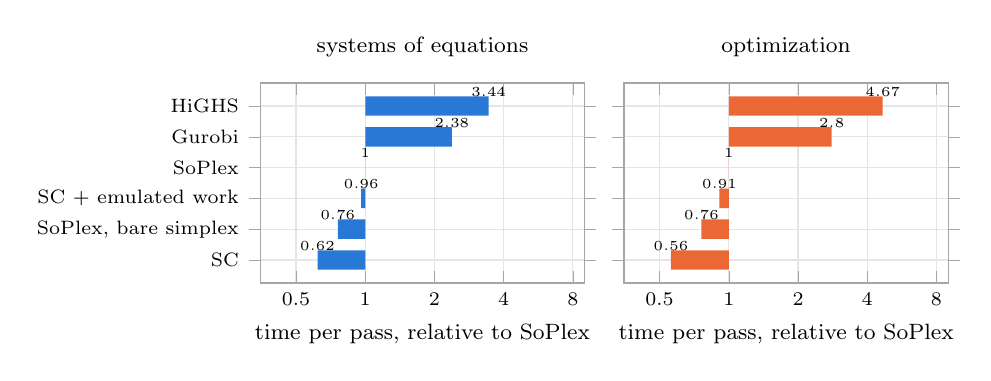
\begin{tikzpicture}
\begin{groupplot}[group style={group size=2 by 1, horizontal sep=0.5cm, yticklabels at=edge left},
  xbar, xmode=log, width=0.47\textwidth, height=0.34\textwidth, /pgf/bar width=7pt,
  xmin=0.35, xmax=9, enlarge y limits=0.15,
  symbolic y coords={SC, {SoPlex, bare simplex}, {SC + emulated work}, SoPlex, Gurobi, HiGHS},
  ytick=data, axis line style={gray!70}, tick style={gray!70}, grid=major, major grid style={gray!20},
  xtick={0.5,1,2,4,8}, xticklabels={0.5,1,2,4,8},
  point meta=rawx, nodes near coords, nodes near coords style={font=\tiny, /pgf/number format/fixed, /pgf/number format/precision=2},
  label style={font=\footnotesize}, tick label style={font=\scriptsize}, title style={font=\footnotesize},
  xlabel={time per pass, relative to SoPlex}]
\nextgroupplot[title={systems of equations}]
\addplot[fill=serieA, draw=none] coordinates {(0.62,SC) (0.76,{SoPlex, bare simplex}) (0.96,{SC + emulated work}) (1.00,SoPlex) (2.38,Gurobi) (3.44,HiGHS)};
\nextgroupplot[title={optimization}]
\addplot[fill=serieB, draw=none] coordinates {(0.56,SC) (0.76,{SoPlex, bare simplex}) (0.91,{SC + emulated work}) (1.00,SoPlex) (2.80,Gurobi) (4.67,HiGHS)};
\end{groupplot}
\end{tikzpicture}
\caption{Time per pass on the bank of Table~\ref{tab:bank}, relative to SoPlex
as used by Ibex (geometric means over the instances). ``SC + emulated work''
is SC with the work of a call of SoPlex added at every LP
(Table~\ref{tab:cascade}); ``bare simplex'' is the simplex of SoPlex driven
directly.}
\label{fig:ladder}
\end{figure}

\subsection{Where the gain comes from}\label{sec:gain}

\paragraph{Inside SC: ablation.}

Table~\ref{tab:ablation} changes one component of SC at a time, inside the search. The pruning
changes little: cell ratios are within 3.5\% in every row. The components
differ in cost, mostly on systems of equations, whose relaxations are larger.
Merging the twin rows is the largest saving (without it, CPU time
$\times1.26$--$1.42$ and eight fewer runs finished), followed by the hybrid
engine (with the tableau alone, $\times1.08$--$1.15$ and seven fewer runs on
systems of equations, $\times1.07$--$1.12$ on optimization problems). The
revised engine alone is about as fast on systems of equations, but 2--3\%
slower on the small relaxations of optimization problems; the
threshold keeps the best of both. Among the pivoting rules, the long-step ratio
test gives 7--10\% on systems of equations, the cost perturbation 3--4\% (and
one more run finished), devex 1--2\%, and the box-scaled tolerance is neutral in
time: it is there for correctness on narrow boxes (Section~\ref{sec:simplex}).
On optimization problems these rules are within 2\%; the perturbation, applied
when the dual warm start relocates the nonbasic variables, does not act there,
and the search is identical without it. Each program loses with the warm start
of the other (Section~\ref{sec:simplex}): the primal warm start is 4--5\%
slower on systems of equations, with one fewer run finished, and the dual
warm start 9--15\% slower on optimization problems. The bound order follows
the warm start: the count read from the tableau saves 1--2\% over the
farthest bound first on systems of equations, where the nearest bound first is
1--2\% slower; on optimization problems the nearest bound first saves 4--5\%
over the farthest and 2--3\% over the count.

\begin{table}[t]
\centering
\caption{Ablation: each row changes one component of SC. Ratios against full
SC: cells and CPU on systems of equations for runs above 0.1, 1 and 5\,s,
runs finished out of 484 (full SC: 364), CPU on optimization problems above
0.1\,s and problems solved in all seeds (full SC: 216). The warm-start row
gives each program the warm start of the other: primal on systems of
equations, dual on optimization problems; the order row gives each the order
of the other: nearest bound first on systems of equations, the count read from
the tableau on optimization problems.}
\label{tab:ablation}
\begin{tabular}{lccccccc}
\toprule
& \multicolumn{5}{c}{systems of equations} & \multicolumn{2}{c}{optimization}\\
\cmidrule(lr){2-6}\cmidrule(lr){7-8}
configuration & cells & $>0.1$\,s & $>1$\,s & $>5$\,s & fin. & CPU & solved\\
\midrule
without cost perturbation         & 1.02 & 1.03 & 1.04 & 1.04 & 363 & 1.01 & 215\\
warm start of the other program   & 1.01 & 1.05 & 1.05 & 1.04 & 363 & 1.09 & 216\\
without long-step ratio test      & 1.01 & 1.10 & 1.08 & 1.07 & 362 & 1.01 & 217\\
without devex                     & 1.01 & 1.01 & 1.02 & 1.00 & 363 & 1.00 & 217\\
without box-scaled tolerance      & 1.00 & 1.01 & 1.00 & 1.00 & 364 & 1.00 & 218\\
tableau engine only               & 1.02 & 1.15 & 1.14 & 1.08 & 357 & 1.07 & 216\\
revised engine only               & 1.00 & 0.99 & 1.00 & 0.99 & 364 & 1.02 & 216\\
without merging twin rows         & 1.02 & 1.42 & 1.34 & 1.26 & 356 & 1.02 & 216\\
farthest-bound order              & 1.00 & 1.02 & 1.02 & 1.01 & 363 & 1.05 & 217\\
order of the other program        & 1.02 & 1.02 & 1.02 & 1.01 & 362 & 1.02 & 217\\
\bottomrule
\end{tabular}
\end{table}

\paragraph{Against SoPlex: emulation.} To attribute the gap with SoPlex we
added to SC, at every LP and on separate vectors, so that its contraction does
not change, each part of the work that SoPlex does in a call, and replayed the
same bank (Table~\ref{tab:cascade}). In logarithmic scale the shares add up. A
refactorization at every LP accounts for 53--58\% of the gap and verifying the
solution for 21--23\%; recomputing the vectors at the start of a solve and
copying the solution add 10--11\%. With everything added, a pass of SC costs
0.91--0.96 times that of SoPlex: these parts explain 84--92\% of the gap, and
the rest is the machinery of a call (setting up and storing vectors, unscaling,
the interface). Driving the simplex of SoPlex directly, which keeps the LP
loaded and verifies nothing, removes 42--54\% of the same gap
(Figure~\ref{fig:ladder}). About half of the difference with SoPlex as used by
Ibex is therefore its interface, and the other half is the refactorization that
its simplex makes before declaring an optimum, which the certificate makes
unnecessary. We also removed parts from SoPlex itself, with a patched copy,
against the default configuration of Ibex, which presolves: there the gap is
larger (SC/SoPlex 0.55 and 0.47), removing the verification accounts for
10--18\% of it, in line with the emulation, and the presolve for 22--23\%.

\begin{table}[t]
\centering
\caption{Attribution of the gap with SoPlex in Table~\ref{tab:bank}: work of
SoPlex added to SC at every LP, cumulatively, as the share of the logarithm of
the time ratio, and the time per pass relative to SoPlex after each step (34
optimization problems: one emulation failed on launch).}
\label{tab:cascade}
\begin{tabular}{lcccc}
\toprule
& \multicolumn{2}{c}{systems} & \multicolumn{2}{c}{optimization}\\
\cmidrule(lr){2-3}\cmidrule(lr){4-5}
step & share & SC/SoPlex & share & SC/SoPlex\\
\midrule
SC                           &      & 0.62 &      & 0.55\\
+ refactorize per LP         & 58\% & 0.82 & 53\% & 0.76\\
+ recompute vectors          &  9\% & 0.85 &  8\% & 0.79\\
+ verify the solution        & 23\% & 0.95 & 21\% & 0.90\\
+ copy the solution          &  2\% & 0.96 &  2\% & 0.91\\
rest of a call               &  8\% & 1.00 & 16\% & 1.00\\
\bottomrule
\end{tabular}
\end{table}

Counting instructions on 200 recorded calls of ex2\_1\_9, with about two
pivots per LP in every engine, gives the same picture at the level of one LP.
A call to SoPlex costs 52 thousand instructions: 32 thousand in its simplex, of
which 10 thousand before the first pivot (setting up the vectors and
refactorizing) and 8 thousand in the pivots themselves; 10 thousand storing and
evaluating the solution, 7 of them verifying it; and the rest in the interface.
Driven directly, the simplex costs 37 thousand per LP. An LP of SC costs 14
thousand, 23 thousand with ordering and certification, and its pivots cost
about the same as those of SoPlex.

\subsection{Where the black box loses bounds}\label{sec:samebox}

With the same certificate, the two engines can only differ in the multipliers
they produce. We ran both engines on the same input boxes and the same polytope
at every node (Table~\ref{tab:samebox}). Two mechanisms appear.
\begin{enumerate}
\item \emph{No optimum.} On some relaxations SoPlex ends without an optimal
basis, and the bound is lost. On Geneig-icse SoPlex reaches the iteration
limit or reports an infeasibility it cannot prove on 379 LPs, against 70 for
SC. (On Brown, before free rows were passed to it empty, SoPlex failed with an
internal exception in 90\% of the LPs; SC solves them all.) SC has no such outcome by design: any basis certifies, and an LP that
stops early yields a weaker bound, not a lost one. With the twin rows unmerged this mechanism was
dominant (a third of the LPs of the black box on Geneig-icse); merging them
removes most of it.
\item \emph{Dual accuracy.} When both engines reach an optimum, the
certificate built from the multipliers of SC is often slightly tighter. On
Geneig-icse, SC contracts more in 128 of 1\,710 nodes and the black box in
9, and on CountercurrentReactors2-9 in 66 against 2; on Bellido and Brown-18
the two engines tie (4 against 4, 1 against 1).
The difference per node is small but compounds along the search; we have not
isolated its cause.
\end{enumerate}
The LPs of SC without an optimum in Table~\ref{tab:samebox} are of another
kind. On Bellido and CountercurrentReactors2-9 they are infeasibility claims of
the warm-started simplex whose ray fails the residual test, 1.1\% and 1.0\% of
its LPs (none reaches the iteration limit); the bound is not contracted and the
pass goes on. At its tolerance of $10^{-6}$ the black box makes no such claim,
but it ends more LPs at an optimum whose certificate does not contract (on
Bellido, 35\% of its LPs against 24\% for SC), which is the second mechanism.

\begin{table}[t]
\centering
\caption{Both engines on the same input boxes and the same polytope. Mean
relative contraction of the perimeter, nodes where each engine contracts more
(nodes that both empty count as ties),
and LPs without a usable certificate (black box with tolerance $10^{-6}$).}
\label{tab:samebox}
\begin{tabular}{lcccccc}
\toprule
& \multicolumn{2}{c}{contraction} & \multicolumn{2}{c}{nodes won} & \multicolumn{2}{c}{LPs not optimal}\\
\cmidrule(lr){2-3}\cmidrule(lr){4-5}\cmidrule(lr){6-7}
system & SC & BB & SC & BB & SC & BB\\
\midrule
Geneig-icse               & 0.323 & 0.323 &  128 &  9 &   70 & 379\\
CountercurrentReactors2-9 & 0.046 & 0.047 &   66 &  2 &  110 &   0\\
Brown-18                  & 0.314 & 0.305 &    1 &  1 &    2 &   0\\
Bellido                   & 0.281 & 0.281 &    4 &  4 &  152 &   0\\
\bottomrule
\end{tabular}
\end{table}

\paragraph{Relation to the polytope-hull contractor of Ibex.}
Against the contractor distributed with Ibex, SC explores about half the
cells on systems of equations. Most of that gap comes from the contractor and
not from the engine: when the LP solver reports infeasibility without a
verifiable ray, the contractor of Ibex abandons the pass, and the node is not
pruned. The black-box engine above, inside our contractor, recovers most of it.

% =====================================================================
\section{Discussion}\label{sec:discussion}

\paragraph{Why SC wins.} SC does not contract with a better polytope: both
engines solve the same relaxation and feed the same certificate. Its advantage
has two sources. The first is cost. On the same LPs a pass of SC costs
0.56--0.62 times that of SoPlex and 0.72--0.80 times that of its simplex driven
directly (Table~\ref{tab:bank}), and SC does not pivot less: it makes 12--36\%
more pivots per LP. What it saves is the work that the certificate makes
unnecessary, a refactorization and a verification at every LP, together with
the setup of a call and the phase~1 that a change of objective or of the box
would otherwise require (Section~\ref{sec:gain}). About half of the gap with
SoPlex as used by Ibex is its interface, and a careful integration of its
simplex recovers it; the other half is in the simplex itself. The second source
is robustness: where the black box ends without an optimum the bound is lost,
while the multipliers of SC still certify it (Table~\ref{tab:samebox}); this is
where the largest gains are (Geneig-icse, DiscreteBoundary-0200), and it does
not depend on how the solver is driven. The slightly tighter certificates of
SC on the remaining LPs compound along the search but are a second-order
effect.

\paragraph{Where it loses.} SC loses where an LP needs many pivots, so that the
cost of a call no longer dominates. Replaying the same sequence of LPs with both
engines, on systems of equations the two need about as many pivots
(Katsurabis-14, 10.0 against 9.1 per LP; Bratu-0060, 7.9 against 10.9), but on
Katsurabis-14 a solve of SoPlex is cheaper (110 against 172\,$\mu$s): with ten
pivots per LP on 30 rows, the pivots of the explicit tableau of SC cost more
than those of the factorized basis of SoPlex. On optimization problems SoPlex
pivots less on some problems (ex6\_2\_10, 1.5 against 2.5 per LP; ex7\_2\_3,
1.3 against 1.9), because it ends 13--40\% of its LPs at a vertex that is
already optimal for the next bound; started at every LP from the final basis of
SoPlex, SC needs about as many pivots as SoPlex on ex2\_1\_9, ex6\_2\_10 and
chem, so the difference lies in the chain of bases and not in the algorithm.
Since an LP of SC still costs a quarter, this matters only where LPs need many
pivots (launch). The third exception of Table~\ref{tab:bank},
DiscreteBoundary-0200, is of another kind: on the same sequence of LPs both
engines need the same pivots (12.4 against 12.7 per LP), and the difference
comes from the LPs that each engine solves in its own pass, with its own order
and skipped bounds. On systems
of equations, SC is slower than the
black box by more than 5\% on three systems. On
the largest relaxations its nodes cost more and it explores slightly more
cells: Bratu-0175 ($\times1.25$, 55 cells against 51) and Bratu-0180
($\times1.12$, 51 against 47); Katsurabis-14 ($\times1.24$) explores the same
cells with costlier nodes. On optimization problems the largest losses are
hhfair1 ($\times1.20$, 1\,596--2\,412 cells against 1\,636--1\,768), concon
($\times1.14$, 2\,444 cells against 1\,690) and ex7\_2\_3 ($\times1.13$), whose
search tree varies by a factor of 4.5 between seeds for SC (17\,902--81\,522
cells; 13\,436--31\,338 for the black box). With the nearest bound first in
both engines, SC loses by more than 5\% only on Katsurabis-14 ($\times1.35$).

\paragraph{What did not pay.} We also measured on the whole benchmark several
ideas that use the certificate or the tableau beyond the pass, and none paid.
Reusing certificates of an ancestor box keeps them valid, by
Proposition~\ref{prop:valid}, but not strong: tested on the slices of ACID,
the multipliers of the node itself almost never prune a slice, and those of an
ancestor prune slices that the linear contractor of the node prunes anyway.
Truncating the LPs with the anytime bound of Proposition~\ref{prop:mono} saves
pivots ($\times0.84$) but weakens the contraction (cells $\times1.39$--$1.60$).
Cuts at the LP optima reduce the cells ($\times0.80$--$0.88$) at a higher cost
(CPU $\times1.18$--$1.31$). A Lagrangian bound improved by monotonicity tightens
the LP bound in most applications, but costs more than it saves (CPU
$\times1.08$ to $\times3.5$). Inheriting the basis between nodes saves pivots
($\times0.78$--$0.96$) but rebuilding the tableau costs as much. Choosing the
warm start of each node by the side changes observed in the previous LPs does
not improve on the choice per program. The pattern is that doing more work
inside a node does not change the search tree; what changed it was what is
computed: the merged relaxation, the stability filter of the ratio test, the
choice of the warm start.

\paragraph{Limits.} SC removes the external LP solver from the contractor, not
from the optimizer: the upper-bounding of IbexOpt still solves its LPs with
SoPlex, in both engines. On problems with very narrow equalities the
upper-bounding becomes the bottleneck: on bearing, whose eight equalities are
relaxed to $|h|\le10^{-8}$, the lower bound of SC is good but feasible points
are found only in boxes of width $10^{-4}$ to $10^{-3}$, and the search tree
changes by two orders of magnitude between seeds; we excluded it, with alkyl
and alkylbis, from the means. Relaxations of several hundred rows are still
expensive for both engines: the systems of 400 to 1\,000 variables of the
benchmark exceed the limits of 60\,s and 6\,GB with either. The cheaper pass of SC comes from
the work per call of a general-purpose solver, whose LPs here need two or three
pivots, not from pivoting less; against the bare simplex of SoPlex the gain of
the whole solver is 7--9\% on optimization problems and 3--5\% on systems of
equations, and SC loses where its LPs need many more pivots than those of
SoPlex (the largest Bratu, Katsurabis-14, launch). On optimization problems SoPlex ends many LPs at vertices that are already
optimal for the next bound, and started from those bases SC needs as few
pivots; neither a tie-break toward the corners of the box inside the optimal
face nor a short walk inside that face (up to ten primal steps that keep the
optimum) made SC end at such vertices, and how to choose them cheaply remains
open.

% =====================================================================
\section{Conclusion}

A polytope-hull contractor solves $2n$ small, closely related LPs per node and
needs a rigorous bound from each. We have shown that the certificate that makes
the bound rigorous, the Neumaier--Shcherbina bound written in the homogeneous
form of the relaxation, is also a design principle for the simplex that
produces it. Since any basis certifies, the simplex needs no verification, no
refactorization before declaring an optimum and no phase~1, and the $2n$
problems share one tableau. Inside the same contractor, with the same
contraction, a pass of this simplex costs 0.56--0.62 times that of SoPlex,
0.72--0.80 times that of its simplex driven directly and 0.12--0.26 times that
of HiGHS and Gurobi, and where the black box loses a bound the simplex still
certifies it. The whole solver is 13--15\% faster on optimization problems and
7--8\% on systems of equations. Two questions remain open: the chain of bases,
since SoPlex ends more LPs at vertices that are already optimal for the next
bound, and the largest relaxations, where the pivots of SC cost more than those
of a factorized basis.

% =====================================================================
\bibliographystyle{plain}
\bibliography{refs}

\end{document}
